\section{Computation}
\subsection{An introduction to algorithms}
An algorithm is a step by step method for solving a problem. It usually includes:
\begin{itemize}
  \item name
  \item brief description
  \item description of input
  \item description of output
  \item sequence of steps to follow
\end{itemize}
Algorithms are often described in \textbf{pseudocode}

\subsubsection*{Assignment operator}
\begin{lstlisting}
  x := y
\end{lstlisting}

\subsubsection*{Return statement}
\begin{lstlisting}
  Return(value)
\end{lstlisting}

\subsubsection*{If-else statement}
\begin{lstlisting}
  If(x = 5), y := 7

  If(condition)             If(condition)
    Step 1                    Step(s)
    Step 2                  Else
    ...                       Step(s)    
    Step n                  End-if
  End-if
\end{lstlisting}

\subsubsection*{For-loop}
\begin{lstlisting}
  For i = s to t    <- first value is s, then s+1, until t is reached
    Step(s)
  End-for
\end{lstlisting}

\subsubsection*{While-loop}
\begin{lstlisting}
  While(condition)
    Step(s)
  End-while
\end{lstlisting}

\subsubsection*{Nested Loops}
\begin{lstlisting}
  Input: sequence a_1, ..., a_n; n

  count := 0
  For i = 1 to n-1
    For j = i+1 to n
      If(a_i = a_j) count := count+1
    End-for
  End-for

  Return(count)
\end{lstlisting}

\subsection{Asymptotic growth of functions}
Consider $f: \mathbb{Z}^+ \rightarrow \mathbb{R}^{\geq}$, where $\mathbb{R}^{\geq}$ denotes the set of non-negative real numbers.
\textbf{Asymptotic growth} of a function $f$ is a measure of how fast the object $f(n)$ grows as the input $n$ grows.
Classification of functions $\mathcal{O}, \Omega,$ and $\Theta$ provide a way to concisely characterize the growth of a function.
\[
  f = \mathcal{O}(g)~~\text{"$f$ is Oh of $g$"}
\]

\subsubsection*{Constant factors}
\begin{align*}
  7n^3 & \rightarrow 7 \text{ is constant factor} \\
  5n^2 & \rightarrow 5 \text{ is constant factor} \\
  3    & \rightarrow 3 \text{ is constant factor}
\end{align*}

\subsubsection*{$\mathcal{O}$ notation}
Let $f$ and $g$ be functions from $\mathbb{Z}^+$ to $\mathbb{R}^{\geq}$.
Then $f=\mathcal{O}(g)$ if there is are positive real numbers $c$ and $n_0$ such that for any $n \in \mathbb{Z}^+$ such that $n \geq n_0$,
\[
  f(n) \leq c \cdot g(n)
\]
Constants $c$ and $n_0$ are said to be a \textit{witness} to the fact $f=\mathcal{O}(g)$

\subsubsection*{$\Omega$ notation}
Let $f$ and $g$ be functions from $\mathbb{Z}^+$ to $\mathbb{R}^{\geq}$.
Then $f=\Omega(g)$ if there is are positive real numbers $c$ and $n_0$ such that for any $n \in \mathbb{Z}^+$ such that $n \geq n_0$,
\[
  f(n) \geq c \cdot g(n)
\]
$f=\Omega(g)$ is read "$f$ is Omega of $g$"

\subsubsection*{Theorem: Relationship of $\mathcal{O}$-notation and $\Omega$-notation}
Let $f$ and $g$ be functions from $\mathbb{Z}^+$ to $\mathbb{R}^{\geq}$. Then $f=\Omega(g) \iff g = \mathcal{O}(f)$

\subsubsection*{$\Theta$ notation}
Let $f$ and $g$ be functions from $\mathbb{Z}^+$ to $\mathbb{R}^{\geq}$.
\[
  f = \Theta(g) \text{ if}: f = \mathcal{O}(g) \land f = \Omega(g)
\]
\begin{itemize}
  \item $f = \Theta(g)$ is read "$f$ is Theta of $g$"
  \item if $f = \Theta(g)$, then $f$ is said to be the \textit{order of} $g$.
\end{itemize}

\subsubsection*{Theorem: Asymptotic Growth of Polynomials}
Let $p(n)$ be a degree-$k$ polynomial of the form
\[
  p(n) = a_{k}n^{k} + a_{k-1}n^{k-1} + \cdots + a_{1}n + a_0 \text{ where } a_k > 0 \\
\]
Then $p(n)$ is $\Theta(n^k)$

\subsubsection*{Asymptotic Growth of Logarithm Functions with Different Bases}
Let $a$ and $b$ be two real numbers greater than 1. Then
\[
  \log_{a}n = \Theta(\log_{b}n)
\]
This is because of the fact that
\[
  \log_{a}n = \log_{a}b \cdot \log_{b}n, \text{ for } a,b > 1
\]
\textit{
  when a function is said to be the $\mathcal{O}$ or $\Omega$ of a logarithm function,
  the base is often omitted because it is understood that as long as the base is greater than 1,
  the value of the base does not matter.
}

\subsubsection*{Growth rate of common functions}
Constant Functions
\begin{itemize}
  \item function that does not depend on $n$ at all
  \item any constant function is $\Theta(1)$
\end{itemize}
Linear
\begin{itemize}
  \item $\Theta(n)$
\end{itemize}
\begin{center}
  \begin{tabular}{l|c}
    Function                                   & Name        \\
    \hline
    $\Theta(1)$                                & Constant    \\
    $\Theta(\log\log n)$                       & Log Log     \\
    $\Theta(\log n)$                           & Logarithmic \\
    $\Theta(n)$                                & Linear      \\
    $\Theta(n \log n)$                         & $n \log n$  \\
    $\Theta(n^2)$                              & Quadratic   \\
    $\Theta(n^3)$                              & Cubic       \\
    $\Theta(n^m)~\text{for}~m\in \mathbb{Z}^+$ & Power       \\
    $\Theta(c^n)~\text{for}~c>1$               & Exponential \\
    $\Theta(n!)$                               & Factorial
  \end{tabular}
\end{center}

\subsubsection*{Rules about Asymptotic Growth}
Let $f$, $g$, and $h$ be functions from $\mathbb{Z}^+$ to $\mathbb{R}^{\geq}$.
\begin{itemize}
  \item if $f=\mathcal{O}(h)$ and $g=\mathcal{O}(h)$, then $f+g=\mathcal{O}(h)$
  \item if $f=\Omega(h)$ and $g=\Omega(h)$, then $f+g=\Omega(h)$
  \item if $f=\mathcal{O}(g)$, $c \cdot f = \mathcal{O}(g)$, $c\in \mathbb{R}^{\geq}$
  \item if $f=\Omega$, $c \cdot f = \Omega(g)$, $c\in \mathbb{R}^{\geq}$
  \item if $f=\mathcal{O}(g)$ and $g=\mathcal{O}(h)$, then $f=\mathcal{O}(h)$
  \item if $f=\Omega(g)$ and $g=\Omega(h)$, then $f=\Omega(h)$
\end{itemize}

\subsection{Analysis of algorithms}
Resources an algorithm requires to run
\begin{itemize}
  \item time, called \textit{time complexity}
  \item space, called \textit{space complexity}
  \item Together called \textbf{computational complexity}
\end{itemize}
\begin{lstlisting}
  ComputeSum
  Input: a_1,a_2,...,a_n  (n is length of sequence)
  Output: the sum of the numbers in the sequence
  sum := 0                  | 1 assignment operation
  For i = 1 to n            | loop iterated n times
    sum := sum + a_i        |   for loop test and increments (2 operations)
  End-for                   |   1 addition and 1 assignment (2 operations)
  Return(sum)               | 1 op for return statement
\end{lstlisting}
\begin{align*}
  f(n) & = 1 + n[2+2] + 1 \\
       & = 1 + 4n + 1     \\
       & = 4n + 2         \\
       & = \mathcal{O}(n)
\end{align*}

\subsubsection*{Growth rates for different input sizes}
\[
  \begin{matrix}
    f(n)       & n=10      & n=50      & n=100                & n=1000                  & \cdots \\
    \log_{2}n  & 3.3 \mu s & 5.6 \mu s & 6.6 \mu s            & 10 \mu s                & \cdots \\
    n          & 10 \mu s  & 50 \mu s  & 100 \mu s            & 1000 \mu s              & \cdots \\
    n\log_{2}n & .03 ms    & .28 ms    & .66 ms               & 10 ms                   & \cdots \\
    n^2        & .1 ms     & 2.5 ms    & 10 ms                & 1 s                     & \cdots \\
    n^3        & 1 ms      & .125 s    & 1 s                  & 16.7 min                & \cdots \\
    2^n        & 1 ms      & 35.7 yrs  & 4 \times 10^{16} yrs & 3.4 \times 10^{287} yrs & \cdots \\
  \end{matrix}
\]

\subsubsection*{Worst-case analysis}
Worst-case analysis evaluates the time complexity on the input which takes the longest time.
\begin{itemize}
  \item upper bound: use $\mathcal{O}$-notation
        \subitem upper bound must apply for every input of size $n$
  \item lower bound: use $\Omega$-notation
        \subitem lower bound need only apply for one possible input of $n$
\end{itemize}
Average-case analysis takes an average running time of algorithm on random inputs.
\begin{lstlisting}
  For(----)
    operations      -> linear (n)
  End-for

  For(----)
    For(----)
      operations    -> quadratic (n^2)
    End-for
  End-for

  For(----)
    For(----)
      For(----)
        operations  -> cubic (n^3)
      End-for
    End-for
  End-for
\end{lstlisting}
and so on. An algorithm runs in \underline{polynomial time} if its time complexity is $\mathcal{O}^k$ for some fixed constant $k$.
An algorithm is considered "efficient" if it runs in polynomial time. For example,
\begin{align*}
  \mathcal{O}(n^5)        & ~\text{is "efficient"}                 \\
  \mathcal{O}(n^{\log n}) & ~\text{is \underline{not} "efficient"}
\end{align*}
\subsection{Finite state machines}
A \textbf{finite state machine} consists of a finite set of states,
with transitions between states triggered by different input actions.
A finite state machine is sometimes called \textit{finite state automation}.
\begin{center}
  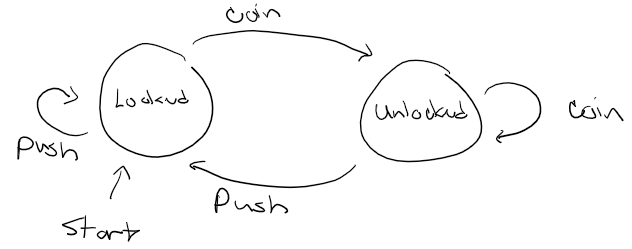
\includegraphics[width=.6\linewidth]{resources/coin_push.png}

  states: $Q =$\{locked, unlocked\}
\end{center}
The reaction of a finite state machine to the input received is denoted by a \textbf{transitive function},
often denoted by the symbol '$\delta$'
\[
  \delta([\text{state}],[\text{action}]) = [\text{state}]
\]
In the case of the coin machine,
\[
  \delta(\text{Locked}, \text{Coin}) = \text{Unlocked}
\]
State transition table:
\begin{itemize}
  \item rows represent current state
  \item columns represent possible inputs
  \item each entry for a particular row and column indicate the new state resulting from that state/input combination
\end{itemize}
For example, the state transition table for the coin machine is
\begin{center}
  \begin{tabular}{c|cc}
             & Coin     & Push   \\
    \hline
    Locked   & unlocked & locked \\
    Unlocked & unlocked & locked
  \end{tabular}
\end{center}

\subsubsection*{Components of a Finite State Machine}
\begin{center}
  \begin{tabular}{c|l}
    Notation                           & Description              \\
    \hline
    $Q$                                & finite set of states     \\
    $q_0 \in Q$                        & $q_0$ is the start state \\
    $I$                                & finite set of actions    \\
    $\delta: Q \times I \rightarrow Q$ & transition function
  \end{tabular}
\end{center}

\subsubsection*{FSM with Output}
\begin{align*}
  Q & = \{q_0, q_5, q_{10}, q_{15}, q_{20}\}                           \\
  I & = \{\text{NICKLE}, \text{DIME}, \text{BUY}\}                     \\
  O & = \{\text{Gumball}, \text{Return}, \text{Message}, \text{None}\}
\end{align*}
\begin{center}
  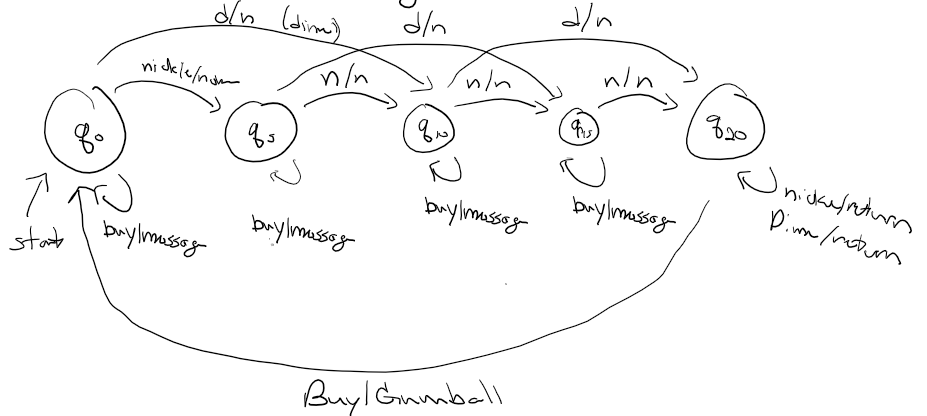
\includegraphics[width=.6\linewidth]{resources/fsm_with_output.png}
\end{center}
An \underline{accepted state} is a state that is okay to end in.
\[
  A \subseteq Q, \text{ Accepted states are a subset of the total states}
\]
Example, recognizing valid password
\begin{center}
  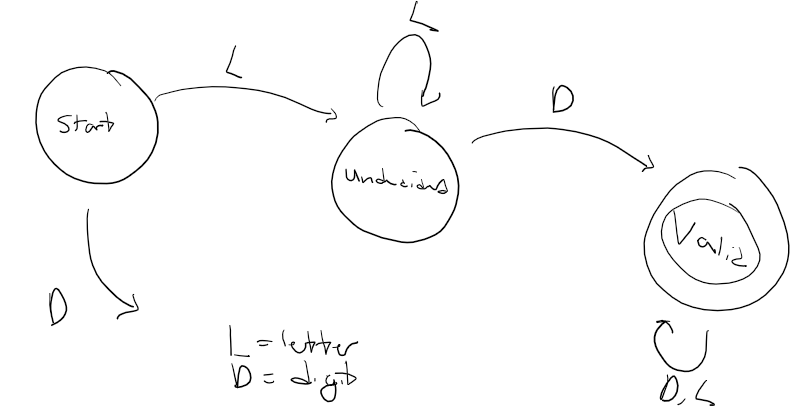
\includegraphics[width=.6\linewidth]{resources/fsm_password.png}

  A valid password must begin with a letter and contain at least one digit.
\end{center}

\subsection{Turing machines}
FSMs are unable to solve even simple computational tasks such as determining whether a binary string has more 0's than 1's.

\subsubsection*{Church-Turing conjecture}
Any problem that can be solved efficiently on any computing device can be solved efficiently by a Turing Machine.

\subsubsection*{Definition of a Turing Machine}
\begin{itemize}
  \item memory is a 1-dimensional tape. \\
        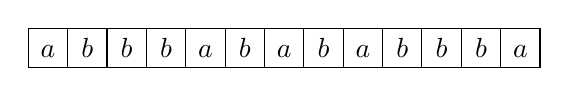
\begin{tikzpicture}
          \pgfmathsetmacro{\x}{0.5}
          \pgfmathsetmacro{\y}{0.5}
          \pgfmathsetmacro{\vset}{0}

          \foreach[count=\i] \element in {a,b,b,b,a,b,a,b,a,b,b,b,a} {
              \draw (\i * \x,0) rectangle ++(\x,\y);
              \node[anchor=south] (\element) at (\i*\x + \x * 0.5, \vset) {$\element$};
            }
        \end{tikzpicture} \\
        example tape for $\{a,b,*\}$
  \item blank symbol (represented by a $*$ symbol)
  \item a \underline{configuration} consists of the contents of the tape, the current state,
        and the tape cell to which the head is currently pointing \\
        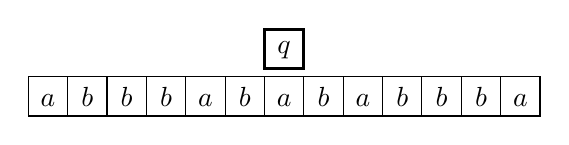
\begin{tikzpicture}
          \pgfmathsetmacro{\x}{0.5}
          \pgfmathsetmacro{\y}{0.5}
          \pgfmathsetmacro{\vset}{0}
          \pgfmathsetmacro{\qset}{7}

          \foreach[count=\i] \element in {a,b,b,b,a,b,a,b,a,b,b,b,a} {
              \draw (\i * \x,0) rectangle ++(\x,\y);
              \node[anchor=south] (\element) at (\i*\x + \x * 0.5, \vset) {$\element$};
            }
          \draw[very thick] (\qset*\x, \y + 0.1) rectangle ++(\x,\y);
          \node[anchor=south] (q) at (\qset*\x + \x*0.5, \y + 0.1) {$q$};
        \end{tikzpicture}
  \item action is determined by a transition function $\delta$
\end{itemize}
Input to Turing Machine is the Input Alphabet, denoted by $\Sigma$,
which much be a subset of the tape alphabet $\Gamma$
\[
  \Sigma \subset \Gamma
\]

\subsubsection*{Components of a Turing Machine}
\begin{center}
  \begin{tabular}{r|l}
    Notation                                                              & Description                                    \\
    \hline
    $Q$                                                                   & finite set of states                           \\
    $\Gamma$                                                              & finite set of tape symbols                     \\
    $\Sigma \subset \Gamma$                                               & A subset of the tape symbols are input symbols \\
    $q_0 \in Q$                                                           & $q_0$ is the start state                       \\
    $q_{acc} \in Q$                                                       & $q_{acc}$ is the accept state                  \\
    $q_{rej} \in Q$                                                       & $q_{rej}$ is the reject state                  \\
    $\delta : Q \times \Gamma \rightarrow Q \times \Gamma \times \{L,R\}$ & Transition Function
  \end{tabular}
\end{center}
Additional Rules
\begin{itemize}
  \item if Turing machine reaches the accept state from a particular input $x$, the Turing machine \textbf{accepts} $x$
  \item if Turing machine reaches the reject state from a particular input $x$, the Turing machine \textbf{rejects} $x$
  \item if Turing machine \textit{accepts} or \textit{rejects} $x$, then the Turing machine \textbf{Halts} on $x$
\end{itemize}
Turing machine that accepts strings with 2 $b$'s
\begin{center}
  \begin{tabular}{c|ccc}
          & $a$         & $b$             & $*$             \\
    \hline
    $q_0$ & $(q_0,a,R)$ & $(q_1,b,R)$     & $(q_{rej},*,L)$ \\
    $q_1$ & $(q_1,a,R)$ & $(q_{acc},b,R)$ & $(q_{rej},*,L)$
  \end{tabular}
\end{center}
\begin{center}
  \begin{tabular}{c}
    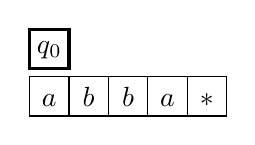
\begin{tikzpicture}
      \pgfmathsetmacro{\x}{0.5}
      \pgfmathsetmacro{\y}{0.5}
      \pgfmathsetmacro{\vset}{0}
      \pgfmathsetmacro{\qset}{1}

      \foreach[count=\i] \element in {a,b,b,a,*} {
          \draw (\i * \x,0) rectangle ++(\x,\y);
          \node[anchor=south] (\element) at (\i*\x + \x * 0.5, \vset) {$\element$};
        }
      \draw[very thick] (\qset*\x, \y + 0.1) rectangle ++(\x,\y);
      \node[anchor=south] (q) at (\qset*\x + \x*0.5, \y + 0.1) {$q_0$};
    \end{tikzpicture} \\
    $\uparrow$ Halts and accepts
  \end{tabular}
  \qquad
  \begin{tabular}{c}
    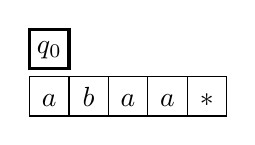
\begin{tikzpicture}
      \pgfmathsetmacro{\x}{0.5}
      \pgfmathsetmacro{\y}{0.5}
      \pgfmathsetmacro{\vset}{0}
      \pgfmathsetmacro{\qset}{1}

      \foreach[count=\i] \element in {a,b,a,a,*} {
          \draw (\i * \x,0) rectangle ++(\x,\y);
          \node[anchor=south] (\element) at (\i*\x + \x * 0.5, \vset) {$\element$};
        }
      \draw[very thick] (\qset*\x, \y + 0.1) rectangle ++(\x,\y);
      \node[anchor=south] (q) at (\qset*\x + \x*0.5, \y + 0.1) {$q_0$};
    \end{tikzpicture} \\
    $\uparrow$ Halts and rejects
  \end{tabular}
\end{center}
Transition function for Turing machine that recognizes powers of 2:
\begin{center}
  \begin{tabular}{c|ccc}
    -           & $a$               & $x$               & $*$               \\
    \hline
    $q_0$       & $(q_{first},*,R)$ & $(q_{rej},*,R)$   & $(q_{rej},x,R)$   \\
    $q_{first}$ & $(q_{even},x,R)$  & $(q_{first},x,R)$ & $(q_{first},*,R)$ \\
    $q_{even}$  & $(q_{odd},a,R)$   & $(q_{even},x,R)$  & $(q_{first},*,R)$ \\
    $q_{odd}$   & $(q_{even},x,R)$  & $(q_{odd},x,R)$   & $(q_{first},*,R)$ \\
    $q_{ret}$   & $(q_{ret},a,R)$   & $(q_{rej},x,R)$   & $(q_{first},*,R)$ \\
  \end{tabular}
\end{center}

\subsection{Decision problems and languages}
\begin{center}
  \begin{tikzpicture}
    %VARIABLES
    \pgfmathsetmacro{\gsize}{1}
    \pgfmathsetmacro{\gnum}{4}

    \foreach[count=\i] \element in {1,2,3,4} { %domain
        \node (\element) at (\i * 360 / \gnum:\gsize) {$\element$};
      }
    \foreach \j/\ls in {1/{2,4},3/{1,4}} {\foreach \l in \ls {\draw[->] (\j) -- (\l);}}
  \end{tikzpicture}
  \begin{tabular}{r|l}
    Symbol set     & ${()~,~;~0~1~2~3~4~5~6~7~8~9}$ \\
    Graph encoding & $4;(1,2)(1,4)(3,1)(3,4)$
  \end{tabular}
\end{center}
Turing Machine can only accept or reject on input.
This limits the class of problems answerable by a turing machine to \textbf{yes} or \textbf{no} problems.
\begin{itemize}
  \item \textbf{Decision Problem}: given a boolean expression, is there
        an assignment to the boolean expression that causes the expression to evaluate to 1?
  \item \textbf{Search Problem}: given a boolean expression, find an assignment to the boolean
        expression that causes the expression to evaluate to 1 if one exists,
        or output that no such assignment exists.
\end{itemize}
If $\Sigma$ is a finite alphabet, then a subset of $\Sigma^*$ is called a \textit{language} over $\Sigma$.

\subsubsection*{Language computed by a Turing Machine}
Let $\Sigma$ denote a finite alphabet and let $L$ be a language over $\Sigma$.
A turing machine $M$ \textbf{computes language L}, or \textbf{decides language L}
if for every $x \in \Sigma$, if $x \in L$, then $M$ rejects $x$ in a finite number of steps.
\begin{itemize}
  \item \textbf{Time Complexity} is measured by how many steps taken by a Turing machine on a particular input.
  \item \textbf{Space Complexity} is measured by the number of tape cells that the turing machine uses in the
        course of it execution on a particular input.
\end{itemize}
A language is \textit{incomputable} if there is no turing machine that computes the language.